\documentclass[10pt,a4paper]{article}
\usepackage[T1]{fontenc}
\usepackage[utf8]{inputenc}
\usepackage{mathptmx}
\usepackage[left=2cm,right=2cm,top=1.6cm,bottom=1.6cm]{geometry}
\usepackage{amsmath,amssymb}
\usepackage{graphicx}
\usepackage{booktabs}
\usepackage{float}
\usepackage{array}
\usepackage{microtype}
\usepackage[font=small,labelfont=bf,skip=4pt]{caption}
\usepackage{titlesec}
\usepackage{enumitem}
\usepackage{xcolor}
\usepackage{listings}
\usepackage[hidelinks]{hyperref}

\titlespacing*{\section}{0pt}{6pt plus 2pt minus 1pt}{3pt}
\titlespacing*{\subsection}{0pt}{5pt plus 1pt minus 1pt}{2pt}
\titleformat{\section}{\normalfont\large\bfseries}{\thesection}{0.6em}{}
\titleformat{\subsection}{\normalfont\normalsize\bfseries}{\thesubsection}{0.6em}{}
\setlist[itemize]{topsep=2pt,itemsep=1pt,parsep=0pt,leftmargin=1.2em}
\setlist[enumerate]{topsep=2pt,itemsep=1pt,parsep=0pt,leftmargin=1.4em}
\setlength{\abovedisplayskip}{4pt}
\setlength{\belowdisplayskip}{4pt}
\setlength{\textfloatsep}{8pt}
\renewcommand{\arraystretch}{1.05}
\linespread{0.97}\selectfont

\lstset{basicstyle=\ttfamily\scriptsize, columns=fullflexible, keepspaces=true,
        breaklines=true, frame=lines, numbers=left, numberstyle=\tiny\color{gray},
        commentstyle=\color{gray}, stringstyle=\color{teal!70!black},
        keywordstyle=\bfseries, showstringspaces=false, upquote=true}

\title{\vspace{-1.2cm}\bfseries The PJS Savings Heuristic for the Team Orienteering Problem:\\
Biased Randomisation and Local Search on the Chao Instances}
\author{Heuristic Algorithms in Transport and Finance --- Master's course assignment \\
    Javier Salvatierra \\
    Jesús Inurria
}
\date{October 2026}

\begin{document}
\maketitle
\vspace{-0.8cm}

\begin{abstract}
\noindent\small
The Team Orienteering Problem (TOP) asks for at most $m$ time-limited routes that collect the largest
total reward from optional customers. We implement in Rust the savings heuristic of Panadero et al.\
(PJS), turn it into a biased-randomised multi-start (GRASP), add a 2-opt and insertion local search on
elite solutions, and test the three layers on the 353 feasible instances of Chao et al.\ (about 2\,min
on a laptop). Over PJS with its best $\alpha$, GRASP adds $7.98\,\%$ to the total reward and
the local search brings the gain to $20.26\,\%$. The mean gap to the best-known solutions is
$2.04\,\%$, or $2.17\,\%$ as Panadero et al.\ measure it, below their $2.85\,\%$ with 128 threads and lower in all seven sets.
Trying 21 values of $\alpha$ pays more than iterating longer with one.
\end{abstract}

\section{Introduction}

A small fleet of $m$ vehicles leaves an origin and must reach a destination before a deadline. On the
way it can visit customers, each with a reward, but there is not enough time to visit them all: the
planner decides which customers to serve, which vehicle serves each of them and in which order. This is the Team
Orienteering Problem (TOP); it maximises the
collected reward instead of minimising distance, and it is NP-hard~\cite{panadero2021}. Panadero et
al.~\cite{panadero2021} adapt the savings of Clarke and Wright~\cite{cw1964} to it, randomise the
heuristic and run it on many threads for one second; Li et al.~\cite{li2022} use it for a dynamic
variant; we study the static TOP with this heuristic, which the course calls \emph{PJS}.

The test data are the classical instances of Chao et al.~\cite{chao1996}: 387 files in seven sets
\texttt{p1}--\texttt{p7}, with 21 to 102 nodes and $m$ between 2 and 4. An instance named
\texttt{p4.3.k} belongs to set 4 (100 nodes: origin, destination and 98 customers), has $m=3$ vehicles,
and the letter \texttt{k} codes the time limit, here $t_{\max}=50$. Within a set the nodes and rewards
are identical; only $m$ and $t_{\max}$ change. In 34 instances no customer fits within $t_{\max}$, so we report on the remaining 353
(the paper speaks of 354). Best-known solutions (BKS) are the column \emph{BEST} of the published results
of PSOiA~\cite{dang2013}; Panadero et al.\ use those of Ke et al.\ quoted in~\cite{panadero2021}, checkable only on the 81
instances of Tables~3--4 of~\cite{panadero2021} (\texttt{p1}--\texttt{p2}), where they coincide with ours.

\section{Problem formulation and enriched savings}
\label{sec:model}

Node $0$ is the origin, node $n+1$ the destination and $N'=\{1,\dots,n\}$ the set of customers; customer
$i$ has a reward $u_i>0$, and $t_{ij}$ is the Euclidean travel time between nodes $i$ and $j$. A route
$R=(i_1,\dots,i_L)$ is travelled as $0\to i_1\to\dots\to i_L\to n+1$, takes
$t(R)=t_{0i_1}+\sum_{k<L}t_{i_ki_{k+1}}+t_{i_L,n+1}$ and collects $u(R)=\sum_{i\in R}u_i$. The TOP reads
\begin{equation}
\max\ \sum_{r=1}^{p} u(R_r)
\qquad\text{s.t.}\qquad
R_r\subseteq N',\quad R_r\cap R_s=\emptyset\ (r\neq s),\qquad p\le m,\qquad
t(R_r)\le t_{\max}\quad (r=1,\dots,p).
\label{eq:model}
\end{equation}
Read literally: at most $m$ routes, no customer served twice, every route within $t_{\max}$, and
customers left out cost nothing.

Joining a route that ends at $i$ with a route that starts at $j$ replaces the legs $i\to n+1$ and $0\to
j$ by the direct leg $i\to j$, which saves the time $s_{ij}=t_{i,n+1}+t_{0j}-t_{ij}$. Unlike in the
vehicle routing problem, this saving depends on the direction and can be negative, because origin and
destination differ in \texttt{p1}--\texttt{p6}: in \texttt{p4.3.k}, $12.8\,\%$ of the 9506 ordered pairs
have $s_{ij}<0$ and $s_{ij}$ ranges from $-19.74$ to $42.57$, whereas in \texttt{p7}, where both depots
coincide, the triangle inequality gives $s_{ij}\ge0$. Panadero et al.\ compute one saving per edge,
arguing that, since travel times are symmetric, the saving does not depend on the
direction~\cite{panadero2021}; with distinct depots the times are still symmetric but the savings are
not, so we keep both directions, as Li et al.\ do~\cite{li2022}. Time alone ignores the objective, so PJS
ranks the pairs by the \emph{enriched saving}
\begin{equation}
s'_{ij}=\alpha\,s_{ij}+(1-\alpha)\,(u_i+u_j),\qquad \alpha\in[0,1],
\label{eq:savings}
\end{equation}
which with $\alpha=1$ counts only time and with $\alpha=0$ only reward (the paper takes
$\alpha\in(0,1)$; our grid includes both ends). Both terms have the same order of magnitude: in
\texttt{p4.3.k} rewards range from 1 to 29, so $u_i+u_j$ lies between 2 and 58.

\section{PJS, GRASP and local search}
\label{sec:method}

\subsection{The PJS heuristic}

Following Section~4 of~\cite{panadero2021}:
\begin{enumerate}
\item \textbf{Dummy solution.} One route $0\to i\to n+1$ per customer. A customer whose dummy route
exceeds $t_{\max}$ is discarded.
\item \textbf{Savings list.} The enriched savings~\eqref{eq:savings} of all ordered pairs are sorted in
decreasing order.
\item \textbf{Merging.} Walking down the list, the arc $(i,j)$ merges the route that ends at $i$ with the
route that starts at $j$ if the result fits in $t_{\max}$; the arc is then deleted, used or not.
\item \textbf{Selection.} Routes are sorted by reward and the best $m$ are kept.
\end{enumerate}
The paper gives no value of $\alpha$, only the rule that it should be close to 0 with heterogeneous
rewards and close to 1 with homogeneous ones~\cite{panadero2021}. The rule does not hold here. Rewards are fixed per set, so there are
only seven values of their coefficient of variation (CV), and over the 285 instances in which $\alpha$
matters the correlation between CV and the best $\alpha$ (the mean of tied optima) is $+0.19$ ($+0.43$ with the
smallest optimum), with the wrong sign either way; in \texttt{p4}, the most heterogeneous set
(CV $0.64$), $\alpha=0$ reaches on average only $68\,\%$ of the best reward over its 54 such instances. In
preliminary trials, not part of the published code, rules based on the CV or on instance features
did not beat a fixed $\alpha$, because the reward jumps irregularly with $\alpha$: a small change reorders the savings list and the greedy merging
builds different routes. We therefore run the 21 values $\alpha=0,0.05,\dots,1$ and keep the best.

\subsection{GRASP: biased-randomised multi-start}

An \emph{iteration} is a complete PJS construction in which the next arc is drawn at random, biased
towards the top of the list. A \emph{run} starts from the deterministic solution, performs iterations in
series and keeps the best, as one thread of Algorithm~1 of~\cite{panadero2021} or the multi-start of
Algorithm~1 of~\cite{li2022}. We test two biased rules:
\begin{itemize}
\item \textbf{Geometric} (the paper's): take the $k$-th remaining arc, $k\sim\mathrm{Geom}(\beta)$ with
$\beta=0.3$~\cite{panadero2021}. Only the position matters.
\item \textbf{Softmax} (our proposal): take each remaining arc with probability proportional to
$\exp(s'_{ij}/\tau)$, $\tau=1$. Arcs with similar savings get similar probabilities.
\end{itemize}

\subsection{Local search on elite solutions}

The local search runs at the end, not inside the iterations, on the \emph{elite} of each instance: the
deterministic solutions of the three best $\alpha$ and, for every $\alpha$ and rule, the best solutions
of the three best runs (ties included); solutions that visit the same customers are kept once. Each
elite solution goes through a loop of two moves: (i)~\textbf{2-opt} inside every route, first improvement;
(ii)~\textbf{insertion} of the unvisited customer with the largest reward that fits somewhere (ties:
least added time) at its cheapest position, repeated while a customer is inserted. No move loses
reward, so no acceptance criterion is needed; the time freed by 2-opt feeds the next insertion.

\section{Implementation}
\label{sec:impl}

The assignment asks for a Python program; we wrote the code in Rust (rustc 1.99, crate
\texttt{pjs} in \texttt{src/rust}) because the experiment consists of 170\,667 independent tasks, which
the library \texttt{rayon} spreads over all threads. The main modules are \texttt{heuristic.rs} (PJS), \texttt{grasp.rs},
\texttt{elite.rs} and \texttt{local\_search.rs}. The savings list is sorted with a \emph{stable} sort,
so tied arcs keep their generation order; ties in the selection step favour the shorter route; and
$t_{\max}$ has a tolerance of $10^{-9}$.

\textbf{Protocol.} For every instance and every $\alpha$: one deterministic construction and 10 runs of
10 iterations with each rule, i.e.\ 21 tasks per $\alpha$ (441 per instance) and 4200 random
constructions per instance. Each run's seed
derives from the base seed 1, the instance, $\alpha$, the rule and the run number, so results are
reproducible bit for bit. On the 81 instances of
Tables~3--4 of~\cite{panadero2021} we also ran, over the 21 $\alpha$, 100 iterations and 1\,s of wall-clock time per run (the
paper's budget; not exactly reproducible), and 20 runs of 1\,s with the best deterministic $\alpha$ only.
The quality measure is $\text{gap}=100\,(\text{BKS}-\text{reward})/\text{BKS}$, averaged over instances; the
paper divides by its own reward instead, which gives slightly larger gaps (our final solutions: $2.17\,\%$
instead of $2.04\,\%$). All runs use 12
threads on an AMD Ryzen 5 5500U laptop (6 cores) under Windows 11; Panadero et al.\ use Java on a 16-core
Xeon (1--128 threads).

\textbf{Validation.} All solutions pass a feasibility check; a separate binary sharing no code re-verifies
the 1000 final routes.

\section{Computational results}
\label{sec:res}

Table~\ref{tab:results} gives the mean gap per set and Table~\ref{tab:p1p2} the comparison on
\texttt{p1}--\texttt{p2}.

\begin{table}[!t]
\centering
\caption{Mean gap to the BKS~\cite{dang2013} per set. \emph{PJS}: best of the 21 $\alpha$;
\emph{GRASP}: best without local search; \emph{Final}: elite + local search (10 iterations);
\emph{Panadero 128}: Figure~4 of~\cite{panadero2021} (BKS of Ke et al., dividing by its own
reward as in its Tables~3--4), \emph{All} weighted by feasible instances; with that denominator
\emph{Final} is 0.60, 0.00, 0.70, 6.38, 1.35, 1.22, 3.61 (\emph{All} 2.17). \emph{Gain}: total reward of Final over PJS.}
\label{tab:results}
\scriptsize
\setlength{\tabcolsep}{4pt}
\begin{tabular}{@{}lrrrrrrrr@{}}
\toprule
 & & Feasible & PJS & GRASP & Final & Panadero 128 & BKS reached & Gain \\
Set & Nodes & instances & gap (\%) & gap (\%) & gap (\%) & gap (\%) & (Final) & (\%) \\
\midrule
\texttt{p1} & 32 & 48 & 6.88 & 3.15 & 0.58 & 0.69 & 40 & 8.70 \\
\texttt{p2} & 21 & 33 & 1.81 & 0.31 & 0.00 & 0.11 & 33 & 2.09 \\
\texttt{p3} & 33 & 60 & 6.84 & 2.96 & 0.67 & 1.44 & 48 & 8.40 \\
\texttt{p4} & 100 & 56 & 29.25 & 23.73 & 5.87 & 7.97 & 5 & 38.75 \\
\texttt{p5} & 66 & 74 & 11.82 & 4.49 & 1.30 & 1.46 & 35 & 13.61 \\
\texttt{p6} & 64 & 24 & 14.45 & 8.51 & 1.17 & 1.42 & 14 & 17.44 \\
\texttt{p7} & 102 & 58 & 19.75 & 14.48 & 3.42 & 5.10 & 14 & 28.07 \\
\midrule
\textbf{All} & & \textbf{353} & \textbf{13.61} & \textbf{8.63} & \textbf{2.04} & \textbf{2.85} & \textbf{189} & \textbf{20.26} \\
\bottomrule
\end{tabular}
\end{table}

\begin{table}[!t]
\centering
\caption{The 81 instances of \texttt{p1}--\texttt{p2}, BKS from Tables~3--4 of~\cite{panadero2021}; all gaps,
those of Panadero et al.\ included, divide by the BKS. \emph{vs.\ P-128}: instances better / equal / worse than Panadero et al.\ with 128 threads; in bold, our
best variant.}
\label{tab:p1p2}
\scriptsize
\begin{tabular}{@{}lrrc@{}}
\toprule
Method & Mean gap (\%) & BKS reached & vs.\ P-128 \\
\midrule
PJS, best $\alpha$ & 4.82 & 44 & 0 / 45 / 36 \\
GRASP, 10 iterations, 21 $\alpha$ & 1.99 & 53 & 1 / 56 / 24 \\
Panadero et al., 1 thread, 1\,s & 1.73 & 52 & --- \\
GRASP, 1\,s per run, 21 $\alpha$ & 0.71 & 65 & 4 / 67 / 10 \\
Panadero et al., 128 threads, 1\,s & 0.44 & 69 & --- \\
GRASP, 10 iterations, 21 $\alpha$ + local search & 0.34 & 73 & 10 / 65 / 6 \\
GRASP, 100 iterations, 21 $\alpha$ + local search & 0.29 & 74 & 12 / 62 / 7 \\
\textbf{GRASP, 1\,s per run, 21 $\alpha$ + local search} & \textbf{0.15} & \textbf{77} & \textbf{12 / 65 / 4} \\
\bottomrule
\end{tabular}
\end{table}

\begin{figure}[!htb]
\centering
\graphicspath{{../results/figures/}}
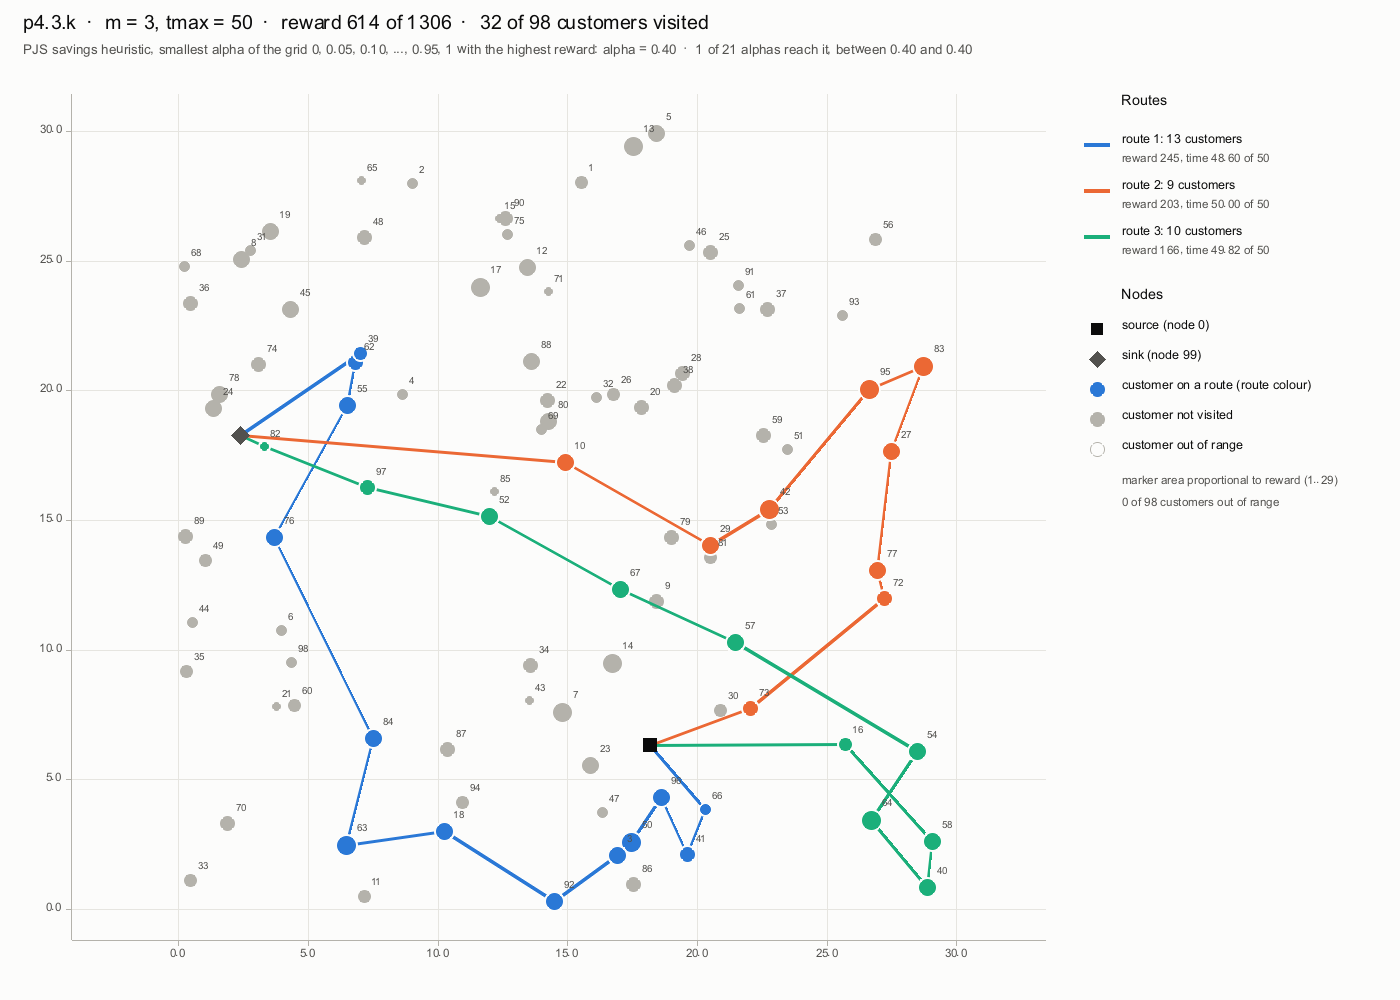
\includegraphics[width=0.45\textwidth,bb=0 0 1400 1000,trim=0 0 340 0,clip]{routes/p4.3.k.png}\hfill
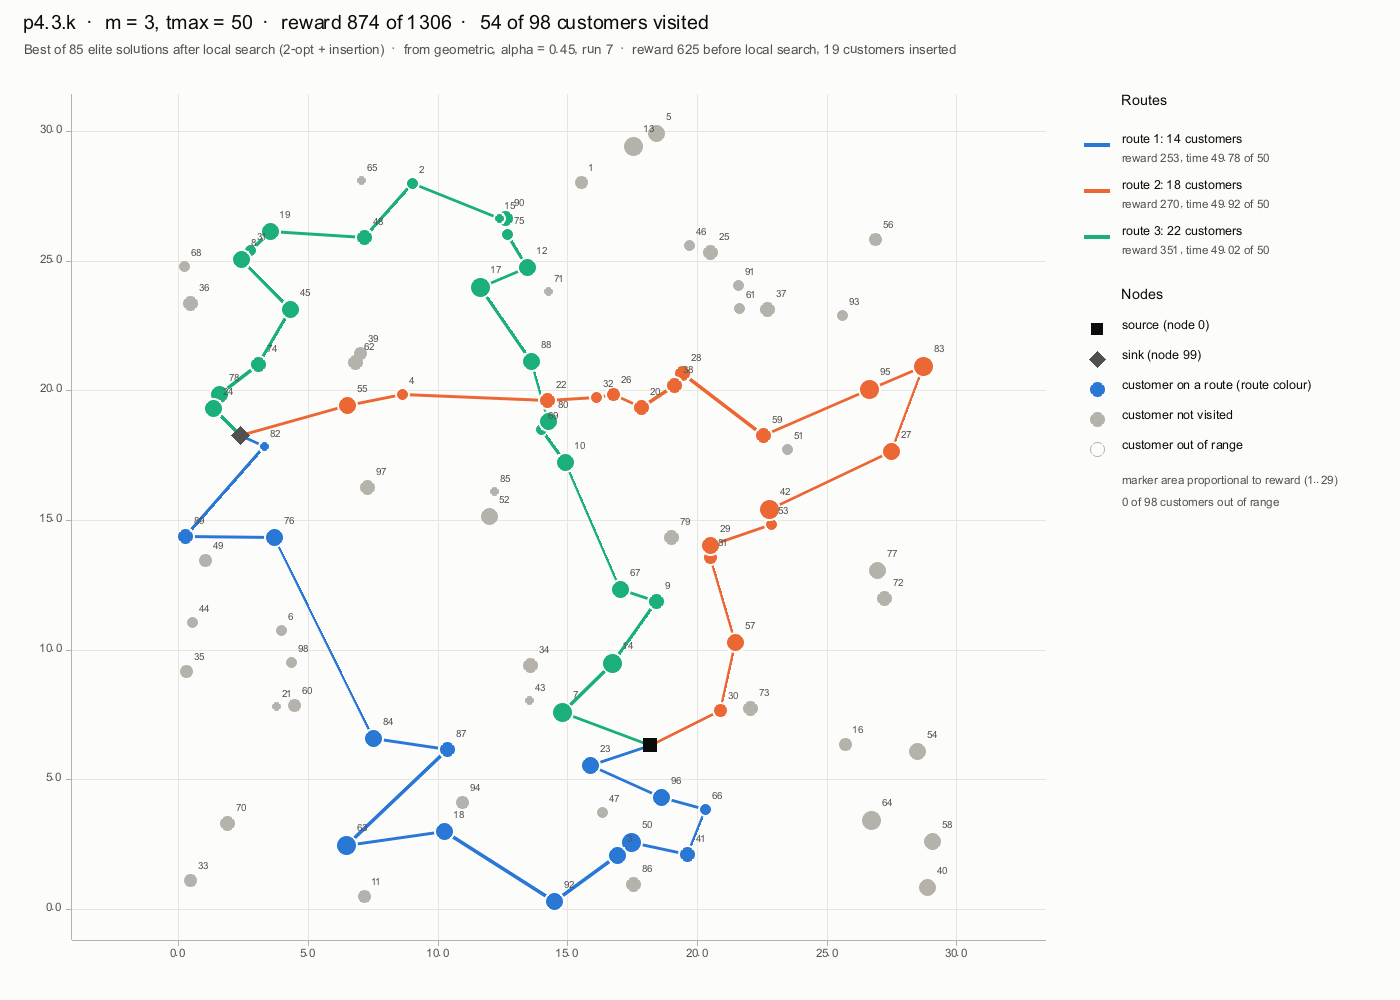
\includegraphics[width=0.45\textwidth,bb=0 0 1400 1000,trim=0 0 340 0,clip]{routes_ls/p4.3.k.png}
\caption{\texttt{p4.3.k} ($m=3$, $t_{\max}=50$; square: origin, diamond: destination; marker size
grows with reward; grey: not visited). Left: PJS with its best $\alpha=0.40$, reward 614 with 32
customers. Right: final solution, reward 874 with 54 customers, from a geometric run with $\alpha=0.45$
worth 625 before the local search, which inserted 19 customers.}
\label{fig:p4}
\end{figure}

\textbf{Each layer adds reward.} Over the 353 instances, PJS with its best $\alpha$ collects 157\,868;
GRASP raises it to 170\,469 ($+7.98\,\%$), the local search on the deterministic elite alone to 181\,103
and on the whole elite to 189\,854 ($+20.26\,\%$), $3.10\,\%$ below the total of the BKS. The local search
raises the reward of an elite solution by $18.16\,\%$ on average (7.48 customers inserted) and improves
$93.6\,\%$ of the 18\,757 elite solutions. The gain grows with the
instance (Table~\ref{tab:results}): $2$--$9\,\%$ in the small sets \texttt{p1}--\texttt{p3}, where few
customers remain outside, and $38.75\,\%$ and $28.07\,\%$ in \texttt{p4} and \texttt{p7}, with about
100 nodes and long routes. Figure~\ref{fig:p4} shows the mechanism: the PJS routes cross the map along
long, almost empty legs, while the final ones sweep dense groups of customers (reward $+42.3\,\%$, from 614 to 874). Diversity matters: in 163 of the 353 instances, applying the local search only to the best
solution before it would have given less (8\,187 reward in total), and on \texttt{p1}--\texttt{p2} the
local search on the deterministic elite alone stops at $2.13\,\%$, against $0.34\,\%$ with the GRASP
elite.

\textbf{Comparison with Panadero et al.} With 10 iterations per run, the final gap is below that of
Panadero et al.\ with 128 threads in all seven sets ($2.17\,\%$ vs.\ $2.85\,\%$ with the paper's denominator), most clearly in
\texttt{p4} and \texttt{p7}. On \texttt{p1}--\texttt{p2} (Table~\ref{tab:p1p2}) it reaches $0.34\,\%$ against
$0.44\,\%$, and $0.15\,\%$ with 1\,s per run (BKS in 77 of 81 instances, worse than the paper in 4). Without the local search no variant reaches the paper's 128 threads, and one of our 1\,s runs gives on
average $2.45\,\%$ (geometric) or $2.33\,\%$ (softmax), worse than the $1.73\,\%$ of one of its threads.
The difference probably lies in what the paper leaves open (tie order, $\alpha$, one or two savings per
edge) and in our runs sharing 6 cores (fewer iterations per run).

\textbf{Many $\alpha$ vs.\ many iterations.} On \texttt{p1}--\texttt{p2}, 1\,s runs with the best
$\alpha$ (on average about 880\,000 constructions per instance, leaving out the trivial \texttt{p2.4.a}) give a
gap of $1.49\,\%$, and 100-iteration runs over the 21 $\alpha$ (42\,000 constructions) give $1.45\,\%$: the same
quality with about 20 times fewer constructions and a fifth of the thread time (4\,s against 20\,s per
instance). Spreading the budget over $\alpha$ explores more.

\textbf{Time.} The grid takes 127\,s on 12 threads for the 387 instances, under 4\,s of thread time per
instance against 128\,s for Panadero et al.\ with 128 threads (different machines and languages, so
only indicative); the local search adds 0.4\,s. The 1\,s variant spends 420\,s of thread time per
instance, so its advantage does not come at equal cost.

\section{Conclusions}

PJS is a greedy pass over a list of enriched savings; even with the best of 21 values of $\alpha$ per
instance it stays $13.61\,\%$ below the best-known solutions. Adding biased
randomisation and a cheap 2-opt and insertion local search on a diverse elite raises the reward by
$20\,\%$ and brings the mean gap to $2.04\,\%$, below Panadero et al.\ with 128 threads in all
seven sets. The large sets \texttt{p4} and \texttt{p7} gain most but remain the weak spot ($5.87\,\%$
and $3.42\,\%$). The next step is a richer neighbourhood (moves between routes, swaps)
inside an iterated local search: diversity first, then repair.

\begin{sloppypar}
\paragraph{Code availability.} \texttt{cargo build -{}-release} in \texttt{src/rust} puts the executable in
\texttt{ignore/target/release}. From \texttt{TOP/}, \texttt{pjs grid data/top-data results} with
\texttt{-{}-png-dir results/figures/routes} and \texttt{-{}-ls-png-dir results/figures/routes\_ls}
reproduces the grid, the local search and Figure~\ref{fig:p4} ($\approx2$\,min); \texttt{pjs bks} and three runs of
\texttt{pjs panadero} (see \texttt{docs/scratchpad.md}) write the CSV files behind Tables~\ref{tab:results}--\ref{tab:p1p2}.
\end{sloppypar}

\begin{thebibliography}{9}
\footnotesize\setlength{\itemsep}{0pt}\setlength{\parskip}{0pt}
\bibitem{panadero2021} J.~Panadero, M.~Ammouriova, A.~A. Juan, A.~Agustin, M.~Nogal and C.~Serrat.
Combining parallel computing and biased randomization for solving the team orienteering problem in
real-time. \emph{Appl.\ Sci.}, 11(24):12092, 2021.
\bibitem{li2022} Y.~Li, M.~Peyman, J.~Panadero, A.~A. Juan and F.~Xhafa. IoT analytics and agile
optimization for solving dynamic team orienteering problems with mandatory visits.
\emph{Mathematics}, 10(6):982, 2022.
\bibitem{cw1964} G.~Clarke and J.~W. Wright. Scheduling of vehicles from a central depot to a number of
delivery points. \emph{Oper.\ Res.}, 12(4):568--581, 1964.
\bibitem{chao1996} I.-M. Chao, B.~L. Golden and E.~A. Wasil. The team orienteering problem.
\emph{Eur.\ J.\ Oper.\ Res.}, 88(3):464--474, 1996.
\bibitem{dang2013} D.-C. Dang, R.-N. Guibadj and A.~Moukrim. An effective PSO-inspired algorithm for the
team orienteering problem. \emph{Eur.\ J.\ Oper.\ Res.}, 229:332--344, 2013.
\end{thebibliography}

\end{document}
